\chapter{Spatial Scheme}
\label{sec:spatial_scheme}

This chapter gives an overview of the available spatial schemes for multiphase flow in \texttt{TRUST}/\texttt{TrioCFD}. First, common notations are given at Section~\ref{sec:notation-spa-sch}. The different schemes of the PolyMAC family are described in Section~\ref{sec:polymac-family}. Few elements are given on the PolyVEF scheme in Section~\ref{sec:polyvef} and on the VDF scheme in Section~\ref{sec:vdf}. Finally, details about the boundary conditions are given in Section~\ref{sec:bounda-condi}.

\section{Notation\label{sec:notation-spa-sch}}
First, we consider a certain polyhedral mesh $\mathtt{M}$. In a three-dimensional framework, $\mathtt{M}$ is composed of different elements: cells $c$, faces $f$, edges $e$ and vertexes $v$. A cell is a peculiar volume subset of the grid. The set of those subsets span the whole grid. A face is defined as the intersection of two cells or the intersection of a cell and a boundary of the domain. An edge is therefore an intersection of faces (and potentially a boundary) and a vertex is the intersection of edges (and potentially a boundary). The total number of each element $\myel$ on the mesh is fixed and will be referred as $\# \myel$. The set of faces of a peculiar cell c will be denoted $F_c$. In the same fashion, the set of edges of a peculiar face $f$ will be noted as $E_f$ and eventually, the two vertexes of an edge $e$ will be denoted $V_e$. 

In the sequel, the measure of an unknown $x$ at an element of the mesh $\myel$ will be denoted: 
\begin{equation}
    [x]_{\myel} = \frac{1}{|\myel|} \int_{\myel} x \, \text{d}\, (\myel)
\end{equation}
where $|\cdot|$ will be a global measure operator of a mesh element. For example, $|c|$ refers to the volume of the cell $c$, $|f|$ to the surface of the face $f$ and $|e|$ to the length of the edge $e$.

Available spatial discretisations in Pb\_multiphase can be seen as extensions of the Marker And Cell (MAC) method \cite{harlow1965numerical} to meshes more complex than Cartesian grids. All those schemes are also available in \texttt{TRUST} \cite{trustonline} for a single phase flow. They are called respectively: VDF, PolyMAC, PolyMAC\_P0, PolyMAC\_P0-P1NC. On the other hand, the PolyVEF\_P0 scheme can be seen as an extension of the Crouzet-Raviart Finite Element scheme.

Compatibility of the available spacial discretisation is summarized in Table~\ref{compatibilteespace}. Please note that only PolyMAC\_P0 and VDF discretisations are currently\footnote{May 2024} validated on multiple test cases. We recommend to use VDF whenever it is possible as computation time is drastically lower than PolyMAC. Figure~\ref{Spatialdiscretisation} succinctly presents the locations of the unknowns for the different discretisations available in Pb\_multiphase.
\begin{table}[!ht]
\begin{center}
\renewcommand{\arraystretch}{1}
   \begin{tabular}{ c  c  c  c  c c  }
     \toprule
     Scheme & PolyMAC & PolyMAC\_P0 & PolyMAC\_P0-P1NC & PolyVEF\_P0P1 & VDF \\
    \midrule
    \rowcolor[gray]{0.9} \texttt{TRUST} & \checkmark & \checkmark & \checkmark & \checkmark  & \checkmark \\ 
     Pb_Multiphase & \xmark & \checkmark & \checkmark & \checkmark & \checkmark \\ 
     \rowcolor[gray]{0.9} Source terms & \xmark & \checkmark & \xmark & \checkmark & \checkmark \\
     Validation & \xmark & \checkmark & \xmark & \xmark & \checkmark\\

     \bottomrule
   \end{tabular}
 \end{center}

\caption{Availability of spatial numerical schemes in Trio_CMFD.}

\label{compatibilteespace}
\end{table}

\begin{figure}[htbp]
  \centering
  \begin{subfigure}[b]{0.45\textwidth}
    %\centering
    
    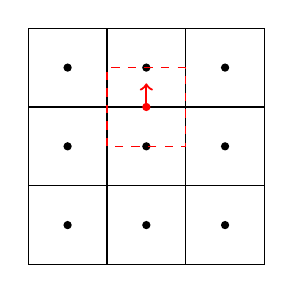
\begin{tikzpicture}[scale=1]
    % mailles
    \foreach \i in {0,1,2}{
      \foreach \j in {0,1,2}{
        \draw (\i,\j) rectangle (\i+1,\j+1);
        % Dessiner un point au centre de chaque maille
        \fill (\i+0.5,\j+0.5) circle (1.5pt);
      }
    }
    
    % Partie rouge
    \draw[->,red,thick] (1.5,2) -- (1.5,2.3);
    \fill[red] (1.5,2) circle (1.5pt);
    \draw[red, dashed] (1,1.5) rectangle (2,2.5);
    
  \end{tikzpicture}
  \caption{VDF MAC.\\ Legend:\\ \textcolor{black}{$\bullet$} $(\alpha, T, P)$ ; \\  
\textcolor{red}{$\bullet$} $(\vec{u} \cdot \vec{n})$, where $\vec{n}$ is the edge normal vector.}
    
    \label{VDF}
  \end{subfigure}
  \hfill
  \begin{subfigure}[b]{0.45\textwidth}
    %\centering
    
    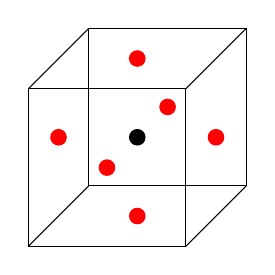
\begin{tikzpicture}[scale=2]
    % cube
    \draw[black] (0,0,0) -- (1,0,0) -- (1,1,0) -- (0,1,0) -- cycle;
    \draw[black] (0,0,1) -- (1,0,1) -- (1,1,1) -- (0,1,1) -- cycle;
    \draw[black] (0,0,0) -- (0,0,1);
    \draw[black] (1,0,0) -- (1,0,1);
    \draw[black] (1,1,0) -- (1,1,1);
    \draw[black] (0,1,0) -- (0,1,1);
    
    
    % face centers
    \foreach \x/\y/\z in {0.5/0.5/0, 1/0.5/0.5, 0.5/0.5/1, 0/0.5/0.5, 0.5/0/0.5, 0.5/1/0.5}
        \fill[red] (\x,\y,\z) circle (1.5pt);
    
    
    % center
    \fill (0.5,0.5,0.5) circle (1.5pt);
    % arrow
  \end{tikzpicture}
  \caption{PolyMAC\_P0. \\ Legend:\\ \textcolor{black}{$\bullet$} $(\alpha, T, P, \vec{u})$ ; \\  
\textcolor{red}{$\bullet$} $(\vec{u} \cdot \vec{n})$, where $\vec{n}$ is the face normal vector.}
    \label{PolyMACP0}
    
  \end{subfigure}
  \vskip\baselineskip
  \begin{subfigure}[b]{0.45\textwidth}
    %\centering
    
      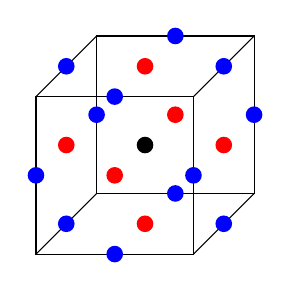
\begin{tikzpicture}[scale=2]
    % cube
    \draw[black] (0,0,0) -- (1,0,0) -- (1,1,0) -- (0,1,0) -- cycle;
    \draw[black] (0,0,1) -- (1,0,1) -- (1,1,1) -- (0,1,1) -- cycle;
    \draw[black] (0,0,0) -- (0,0,1);
    \draw[black] (1,0,0) -- (1,0,1);
    \draw[black] (1,1,0) -- (1,1,1);
    \draw[black] (0,1,0) -- (0,1,1);
    
    
    % face centers
    \foreach \x/\y/\z in {0.5/0.5/0, 1/0.5/0.5, 0.5/0.5/1, 0/0.5/0.5, 0.5/0/0.5, 0.5/1/0.5}
        \fill[red] (\x,\y,\z) circle (1.5pt);
    
    % edge centers
    \foreach \x/\y/\z in {0.5/0/0, 1/0.5/0, 0.5/1/0, 0/0.5/0, 0/0/0.5, 1/0/0.5, 1/1/0.5, 0/1/0.5, 0.5/0/1, 1/0.5/1, 0.5/1/1, 0/0.5/1}
        \fill[blue] (\x,\y,\z) circle (1.5pt);
    
    % center
    \fill (0.5,0.5,0.5) circle (1.5pt);
    % arrow
  \end{tikzpicture}
  \caption{PolyMAC\_P0-P1NC. \\ Legend:\\ \textcolor{black}{$\bullet$} $(\alpha, T, P, \vec{u})$ ; \\  
\textcolor{red}{$\bullet$} $(\vec{u} \cdot \vec{n}, T_{aux}, P_{aux})$, where $\vec{n}$ is the face normal vector ; \\ \textcolor{blue}{$\bullet$} $\vec{curl}(\vec{u}).\vec{t}$, where $\vec{t}$ is the edge tangent vector.}
    
    
    \label{PolyMACP0P1NC}
  \end{subfigure}
  \hfill
  \begin{subfigure}[b]{0.45\textwidth}
    %\centering
    
    
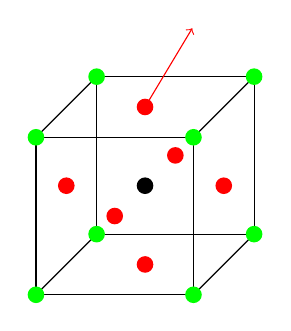
\begin{tikzpicture}[scale=2]
    % cube
    \draw[black] (0,0,0) -- (1,0,0) -- (1,1,0) -- (0,1,0) -- cycle;
    \draw[black] (0,0,1) -- (1,0,1) -- (1,1,1) -- (0,1,1) -- cycle;
    \draw[black] (0,0,0) -- (0,0,1);
    \draw[black] (1,0,0) -- (1,0,1);
    \draw[black] (1,1,0) -- (1,1,1);
    \draw[black] (0,1,0) -- (0,1,1);
    
    % vertices
    \foreach \x/\y/\z in {0/0/0, 1/0/0, 1/1/0, 0/1/0, 0/0/1, 1/0/1, 1/1/1, 0/1/1}
        \fill[green] (\x,\y,\z) circle (1.5pt);
    
    % face centers
    \foreach \x/\y/\z in {0.5/0.5/0, 1/0.5/0.5, 0.5/0.5/1, 0/0.5/0.5, 0.5/0/0.5, 0.5/1/0.5}
        \fill[red] (\x,\y,\z) circle (1.5pt);
    
    
    % center
    \fill (0.5,0.5,0.5) circle (1.5pt);
    % arrow
    \draw[->,red] (0.5,1,0.5) -- ++(0.3,0.5,0);
  \end{tikzpicture}
  \caption{PolyVEF_P0P1. \\ Legend:\\ \textcolor{black}{$\bullet$} $(\alpha, T, P)$ ; \\  
\textcolor{red}{$\bullet$} $\vec{u}$ ; \\ \textcolor{green}{$\bullet$} $(\alpha,T,P)$.}    
    
    \label{PolyVEF}
  \end{subfigure}
  \caption{Scheme of different storing locations for each discretisation available in Pb\_multiphase.}
  \label{Spatialdiscretisation}
\end{figure}

\section{The PolyMAC family\label{sec:polymac-family}}
As stated above, the PolyMAC discretisation's family aims to extend the MAC scheme to complex polyhedral and deformed grids. Indeed, staggered discretisation tends to decrease the appearance of potential spurious mode in low Mach number regime. PolyMAC are based on Finite Volumes methods. As such, unknown are discretised and stored on control volumes. Moreover, for each PolyMAC method, a dual mesh (more or less complex depending on the PolyMAC version) is constructed and operators are defined in order to interpolate unknowns from a control volume to another (face to edge, vertex to cell, \ldots). Those scheme are also available in \texttt{TRUST} code for solving the incompressible Navier-Stokes system. In practice, the discretisation methods are coded in \texttt{TRUST} in a modular fashion, so that they can be used for various models. 

\subsection{PolyMAC}
The first developed PolyMAC version, simply called PolyMAC in \texttt{TRUST}/\texttt{TrioCFD}, is based on a \textit{mimetic} method~\cite{lipnikov2014mimetic}. The core idea of those methods is to conserve exact property at the discrete level. To be more precise, PolyMAC lays in the \textit{Compact Discrete Operator} framework, such as the one presented by \textcite{bonelle2014,milani2020}. A dual mesh has to be build and unknown and equations are discretised on this dual mesh. In this framework, local quantities are discretised according to their physical properties. This leads to exact discrete operator such as the gradient, curl and divergence. Some other approximated interpolation operators, called Hodge operators, must also be defined.

However, up to know, this version is not available in Pb\_multiphase as the discretisation of the two-phase flow model leads to a non-triangular matrix (because of the use of the vorticity) and two saddle point problems that impair greatly the stability and performance of the computation in the multiphase flow framework. 

\subsection{PolyMAC\textunderscore{}P0}
Unlike the first PolyMAC discretisation, PolyMAC\_P0 is not based on a CDO approach and the discretisation does not require explicitly a dual mesh. Moreover, in this case, equations are discretised at the control volume of their principal unknown: $\alpha _k \rho _k$ for $\mathcal{M}_k$, $u_k$ for $\mathcal{Q}_k$ and $T_k$ for $\mathcal{E}_k$.

\subsubsection{Discretisation of the unknown}
For $k \in \{1,2\}$:
\begin{itemize}
    \item the velocity $ u_k $ is discretised by the average of its outer-pointing normal component at the face:
    \begin{equation}
        [u_k] _f = \frac{1}{|f|} \int _f \vec{u_k} \cdot \vec{n_f} \,  dS,
    \end{equation}
    with $\vec{n_f}$ a unit outer-pointing normal of the face $f$.
    \item The pressure P is discretised over the cell:
    \begin{equation}
        [P]_c = \frac{1}{|c|} \int _c p dV,
    \end{equation}
    \item the temperature $T_k$ is discretised over the cell:
    \begin{equation}
        [T_k]_c = \frac{1}{|c|} \int _c T_k dV,
    \end{equation}
    \item the partial fraction $ \alpha _k$ is discretised over the cell:
    \begin{equation}
        [\alpha _k]_c = \frac{1}{|c|} \int _c \alpha _k dV,
    \end{equation}
\end{itemize}
\subsubsection*{Discretisation of gradient terms}
For PolyMAC\_P0, the reconstruction of the gradient at the face is conducted through a Multi Point Flux Approximation (MPFA) method \cite[section 4.1]{droniou2018gradient}. Those methods gives approximations of the gradient at the face, called $G^{\text{MPFA}}$ (see sub-section \ref{MPFA_gradient_subsec} for its definition). However, gradient of a scalar field $\mathcal{F}_s$ at the cell center will be needed in the following. Its value is thus interpolate by using the following operator taken from \textcite{bonelle2014}:
\begin{equation}
    \croc{\vec{\nabla F_s}}_c = \frac{1}{|c|} \sum _{f \in F_c} |f| [u]_f |\nabla  \mathcal{F}_s |_f \vec{x}_{c \rightarrow f},
\end{equation}
where $\vec{x}_{c \rightarrow f}$ is the vector linking the gravity center of the cell $c$ to the gravity center of the face $f$.

\subsubsection{Discretisation of the scalar equations}
First, we want to take care of the scalar equations. Those equations, \textit{i.e.} for $k\in \{1,2\} $ ($\mathcal{M}_k$) and ($\mathcal{E}_k$), are discretised at the cell. Considering a scalar field $\mathcal{F}_s$, then, owing to the Stokes theorem, we have:
\begin{equation}
    |c| [\nabla \cdot (F_s \vec{u})]_c = \sum _{f \in F_c} |f| [\mathcal{F}_s]_f [u]_f \label{disc_div_polyp0}
\end{equation}
The scalar fields at the face are reconstructed from their values at the cell by using an upwind reconstruction. Equation \eqref{disc_div_polyp0} is used to discretised every divergence terms in the scalar equations. 

\subsubsection*{Discretisation of the momentum equation}

The momentum equation ($\mathcal{Q}_k$) is discretised at the faces. However, as it is challenging to construct a discretisation of convective terms $\nabla \cdot (\alpha _k \rho _k \vec{u}_k \otimes \vec{u}_k)$ and diffusives terms $[\nabla \cdot (\alpha_k \mu _k (\vec{\nabla} \vec{u}_k) + (\vec{\nabla} \vec{u}_k)^\intercal) ]$ with only the velocity projected at the face, the following method is used:
\begin{itemize}
\item For convective terms:
  \begin{enumerate}
  \item Approximate the value of the velocity at the cells in the same manner as the gradient:
    \begin{equation}
      [\vec{u}]_c = \frac{1}{|c|} \sum _{f \in F_c} |f| [u]_f \vec{x}_{c \rightarrow f}.
    \end{equation}
  \item Discretise the convective terms at the cell centers:
    \begin{align}
      [\nabla \cdot ( \alpha _k \rho _k \vec{u}_k \otimes \vec{u}_k)]_c &= [\alpha _k \rho _k]_c [\nabla \cdot ( \vec{u}_k \otimes \vec{u}_k)]_c \\
                                                                        &= \frac{[\alpha _k \rho _k]_c}{|c|} \sum _{f \in F_c} |f| [\vec{u}_k \otimes \vec{u}_k]_f \\
                                                                        &\simeq \frac{[\alpha _k \rho _k]_c}{|c|} \sum _{f \in F_c} |f| [u]_f \left( \beta \left( \gamma \vec{u_c} + \left(1-\gamma \right) \vec{u_{c'}} \right) \right. \notag \\ & \quad \left. + (1-\beta) \left( \frac{\vec{u_c} +\vec{u_{c'}}}{2} \right) \right),
    \end{align}
    with $\beta \in [0,1]$ and $\gamma \in \{0,1\}$ such that $\gamma =1$ if $[u_f]\geq 0$ and $0$ otherwise. When taking $\beta =0$, the staggered scheme is retrieved, and when taking $\beta =1$, we retrieved the upwind scheme (used by default in PolyMAC\_P0).
  \item Interpolate convective terms to the face:
    \begin{equation}
      [\nabla \cdot (\alpha _k \rho _k \vec{u}_k \otimes \vec{u}_k)]_f = \lambda_{c,f} [\nabla \cdot (\alpha _k \rho _k \vec{u}_k \otimes \vec{u}_k)]_c + \lambda_{c',f} [\nabla \cdot (\alpha _k \rho _k \vec{u}_k \otimes \vec{u}_k)]_{c'}
    \end{equation}
    with the penalty coefficient $\lambda_{c,f} = \frac{ |\vec{x}_{c' \rightarrow f}|}{|\vec{x}_{c' \rightarrow f}| + |\vec{x}_{c \rightarrow f}|}$, with $c'$ the neighbouring cell of $c$ sharing the face $f$.
  \end{enumerate}
\item For diffusive terms:
  \begin{enumerate}
  \item Approximate the velocity $u_k$ at the cell using a second order method:
    \begin{equation}
      [\vec{u}]_c = \frac{1}{|c|} \sum _{f \in F_c}  (\vec{\alpha} _f + \vec{\beta} _f)[u]_f ,
    \end{equation}
    where $\vec{\alpha}_f = |f| \vec{x}_{c \rightarrow f}$ and $\vec{\beta}$ is a vector which component depends on $\vec{x}_{c' \rightarrow f'}$. Vector $\vec{x}_{c' \rightarrow f'}$ links the gravity center of the neighbour cells $c'$ of $c$ to the gravity center of the face $f'$ of $c'$ which have a common vertex with $c$. Vector $\beta_f$ is computed through the minimisation of a function.
  \item Compute:
    \begin{equation}
    \begin{aligned}
      [\nabla \cdot (\alpha_k \mu _k (\vec{\nabla} \vec{u}_k) + (\vec{\nabla} \vec{u}_k)^\intercal) ]_c = \sum_{\tilde{f}} |\tilde{f}| [\alpha_k]_c [\rho_k]_c & (G^{\text{MPFA}} ([u]_c) \\ &+ \left(G^{\text{MPFA}} ([u]_c))\right) ^\intercal \cdot \vec{n}_f.
    \end{aligned}
    \end{equation}
    
  \item Interpolate diffusive terms to the face:
    \begin{equation}
      \begin{split}
        [\nabla \cdot (\alpha_k \mu _k (\vec{\nabla} \vec{u}_k) + (\vec{\nabla} \vec{u}_k)^\intercal) ]_f =&  \lambda_{c,f}  [\nabla \cdot (\alpha_k \mu _k (\vec{\nabla} \vec{u}_k) + (\vec{\nabla} \vec{u}_k)^\intercal) ]_c \\ &+ \lambda_{c',f}  [\nabla \cdot (\alpha_k \mu _k (\vec{\nabla} \vec{u}_k) + (\vec{\nabla} \vec{u}_k)^\intercal) ]_{c'}
      \end{split}
    \end{equation}
  \end{enumerate}
\end{itemize}


The other terms of ($\mathcal{Q}_k$) are simply constructed by using the Stokes theorem, the velocity at the face and MPFA methods.

Remark: \textit{ Point 3 for reconstruction at the face of convective and diffusive terms can lead to a stability issue on very deformed grids.  } 


\subsection{MPFA methods: gradient approximations} \label{MPFA_gradient_subsec}
In \texttt{TRUST} code, three version of MPFA for gradient reconstruction exist: MPFA-O \cite{AgMa08}, MPFA-O(h) \cite{edwards1998finite} and MPFA-symmetric \cite{Lepot05}. In practice, the choice of the MPFA method follow this algorithm:

\begin{algorithm}[H]
  \SetAlgoLined
  \KwIn{A cell $c$}
  \KwOut{MPFA\_scheme}
  \BlankLine
  \textbf{Step 1: Test of the stability condition \eqref{MPFA_stability_cdt} on $c$ using a MPFA-O method}\;
  \uIf{\eqref{MPFA_stability_cdt}==TRUE}{
    MPFA\_scheme=MPFA-O\;
    break\;
  }
  \textbf{Step 2: Test of the stability condition \eqref{MPFA_stability_cdt} on $c$ using a MPFA-O(h) method}\;
  \uIf{\eqref{MPFA_stability_cdt}==TRUE}{
    MPFA\_scheme=MPFA-O(h)\;
    break\;
  }
    MPFA\_scheme=MPFA-symmetric\;
    break\;
  \caption{Selection of the MPFA method}
\end{algorithm}

The first one is more precise but less stable than the second one which is respectively more precise and less stable than the third one. The MPFA-symmetric method can always be computed but can lack in consistency on very deformed mesh. MPFA-O \cite{AgMa08} and MPFA-O(h) methods have a stability condition which ensures that they stay coercive, see \eqref{MPFA_stability_cdt}. 
A detailed introduction to MPFA methods can be found in \cite{droniou2014finite}. Those methods are considered as gradient approximation methods, see \cite[section 4.1]{droniou2018gradient}. 

In the sequel, we will present the MPFA-O method.

In this case, in order to compute the gradient approximation, a dual mesh is constructed. It can be seen on Figure~\ref{MPFA} in the case of a triangular mesh. The primal mesh vertexes are represented by \textcolor{red}{\textbullet} in Figure~\ref{MPFA}. The procedure to build the dual mesh is:
\begin{itemize}
    \item Link each cell's ($c$) gravity center (\textcolor{black}{\textbullet} in Figure \ref{MPFA}) to the gravity center of each cell's face $f \subset c$ (\textcolor{Blue}{\textbullet} in Figure \ref{MPFA}). Doing so, the face of the mesh are cut into two sub-faces called $\tilde{f}_1$ and $\tilde{f}_2$. Each cell can then be subdivided into $N_i$ quadrilaterals, called $(S_{c,i})_{i\in\{ 1,\dots, N_i \} } $ in Figure \ref{MPFA}.
    \item Introduce inside each sub-face $\tilde{f} \subset f$, an auxiliary quantity (\textcolor{Green}{\textbullet} in Figure \ref{MPFA}). For MPFA-symmetric method, those auxiliary quantities are set at one third and two third of the face $f$.
\end{itemize}
\noindent  On $S_1$ in Figure \ref{MPFA} for example, the gradient of a potential p, $G_{S_{c,i}}([p]_c)$ is computed as:
\begin{equation}
    G_{S_{c,i}}([p]_c) = \frac{1}{|S_{c,i}|} ( (p_{S_{c,1},1} -p_c)  \vec{n_1} + (p_{S_{c,1},2} -p_c)  \vec{n_2} ),
\end{equation}
where $\vec{n_1}$ and $\vec{n_2}$ are the outward unit normal vectors of the respective sub-faces $\tilde{f}\subset f$ where the auxiliary elements $p_{S_{c,1}}$ and $p_{S_{c,2}}$ are located.
Thus, $G^{\text{MPFA}}$ writes:
\begin{equation}
    G^{\text{MPFA}}: [p]_c \mapsto G^{\text{MPFA}}([p]_c) \ , \quad \forall c \in C \ , \quad i \in S_c \ : \quad G^{\text{MPFA}} _{|S_{c,i}} =  G_{S_{c,i}}([p]_c).
\end{equation}
A core assumption of the MPFA method is to suppose that $G^{\text{MPFA}}([p]_c)$ is constant on each $S_{c,i}$. 

When enforcing the continuity across the sub-faces that are linked by a vertex of the primal mesh, auxiliary variables can be substitute by cells unknowns. 

By construction, this approach guarantees local flux imbalance.
\begin{figure}
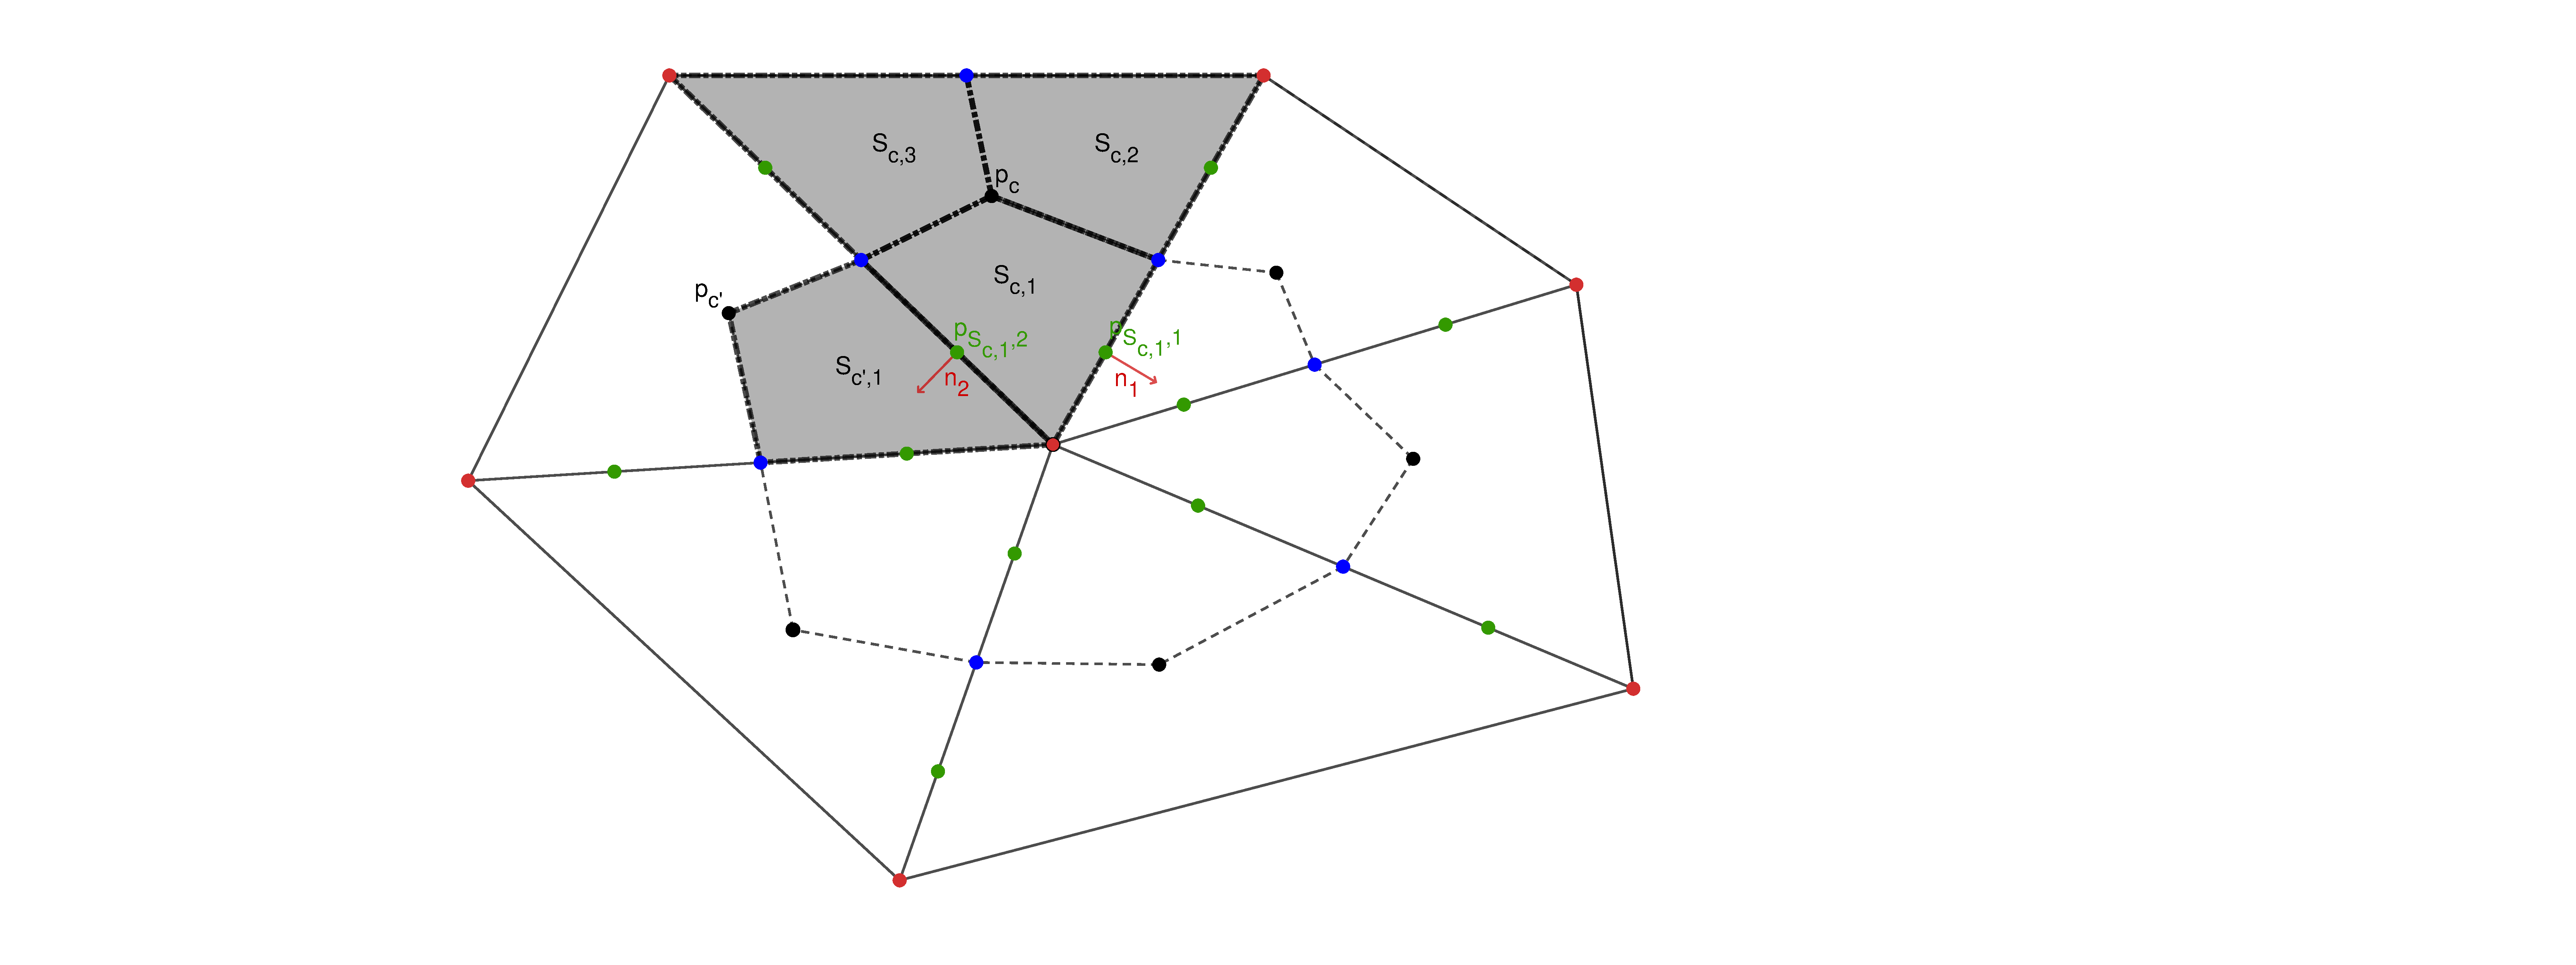
\includegraphics[scale=0.2]{Figure/MPFAPolymac1.pdf}
\caption{Scheme of the MPFA method for a triangular mesh \cite{Bacq}.}
\label{MPFA}
\end{figure}

For a face $f$ of vertex $i$ and $j$, shared by cells $c$ and $c'$, the \textbf{stability condition} of the MPFA method reads:
\begin{equation}
    \forall (k,l) \in \{i,j\}, \ \forall (\tilde{c},\hat{c})\in \{c,c' \}, \ G_{S_{\tilde{c},k}} \cdot G_{S_{\hat{c},l}} \geq 0 \label{MPFA_stability_cdt}
\end{equation}

Some remarks:
{
\it
\begin{itemize} 
    \item  Due to large stencil of the MPFA scheme induced by the elimination of the auxiliary unknows, PolyMAC\_P0 tends to be more costly when using tetrahedron grids rather than hexahedron grids.
    \item  On the boundary of the domain, only one auxiliary quantity is constructed by face when no Dirichlet or Neumann are imposed. 
\end{itemize}
}

\subsection{PolyMAC\textunderscore{}P0-P1NC}
The PolyMAC\_P0-P1NC discretisation aims at reducing some stability issues of PolyMAC\_P0. It uses an Hybrid Finite Volume method described in \cite{eymard2007} in the case of a diffusion problem. Moreover, as in the first PolyMAC discretisation, the vorticity $\omega = \nabla \wedge u$ is introduced. We remind that no source terms are implemented and no validation have been made for this scheme. We do not recommend to use this scheme for most cases.

\section{PolyVEF\textunderscore{}P0\label{sec:polyvef}}
The PolyVEF\_P0 discretisation method is different from the PolyMAC family. Indeed, it is an extension to arbitrary polyhedron of the Crouzeix-Raviart Finite Element Method named VEF in \texttt{TRUST}/\texttt{TrioCFD}, hence the name PolyVEF. In this case, scalar quantities are stored at the cell and at the vertexes. However, the entire velocity vector is stored at the face as described in Figure~\ref{PolyVEF}. As in PolyMAC\_P0, the gradient is reconstructed by using MPFA methods. 
However, time schemes ICE and SETS are not sufficient for using PolyVEF\_P0. We remind that no validation have been made for this scheme and that it is not available in the TRUST environment. We do not recommend to use this scheme for most cases.

\section{VDF\label{sec:vdf}}
This discretisation method is designed to be compatible with conforming meshes composed of hexahedral elements. It is a conservative Finite Volume scheme of MAC \cite{harlow1965numerical} type.
All scalars are stored at the center of each control volume when the velocity field which is defined on a staggered mesh. It is summarized on Figure~\ref{VDF}. It must be emphasised that a hexahedral mesh is not considered being a cartesian mesh. In practise, hexahedral grids are not always cartesian.

This discretisation allows 2D axi-symetrical configurations. It can be activated using the keyword \texttt{bidim\_axi}.

\section{Boundary conditions\label{sec:bounda-condi}}
An object called a boundary condition is used to define, for a given equation, the conditions to be applied on a domain's boundary. Each boundary condition object contains a reference to the \texttt{Domain\_Cl\_dis\_base} object to which it belongs. Each object also contains a \texttt{Champ\_front} object containing the values to be imposed on the boundary.
The main \texttt{Champ\_front} used are summarized in the following table \ref{Champfront}. 

\begin{table}[!ht]
    \centering
       \begin{tabular}{c c  c }
        \toprule
        Keyword & Steady & Uniform \\
        \midrule
        \rowcolor[gray]{0.9} \texttt{champ_front_uniforme} & \checkmark & \checkmark  \\
        \texttt{champ_front_fonc_xyz} &  \checkmark & \xmark \\
        \rowcolor[gray]{0.9} \texttt{champ_front_fonc_t} & \xmark &  \checkmark \\
        \texttt{champ_front_fonc_txyz} & \xmark & \xmark \\
        \bottomrule
    \end{tabular}
    \caption{Main Champ_front for boundary conditions.}
    \label{Champfront}
\end{table}

In multiphase problems \texttt{champ\_front\_composite} can be used to associate different boundary conditions to each phase. For example:
\begin{lstlisting}
champ_front_composite 2
{
    champ_front_uniforme 3 0 0 1
    champ_front_uniforme 3 0 0 1
}
\end{lstlisting}
A special \texttt{Champ\_Front\_MUSIG} associated with \texttt{Milieu_MUSIG} can be used to give boundary conditions to each phase. For example: 
\begin{lstlisting}
Champ_Front_MUSIG {
    nbPhases 1 Champ_Front_Uniforme 1 0.03 # Gas 0 #
    nbPhases 1 Champ_Front_Uniforme 1 0.04 # Gas 1 #
    nbPhases 1 Champ_Front_Uniforme 1 0.05 # Gas 2 #
    nbPhases 1 Champ_Front_Uniforme 1 0.07 # Gas 3 #
    nbPhases 1 Champ_Front_Uniforme 1 0.03 # Liquid 0 #
    nbPhases 1 Champ_Front_Uniforme 1 0.05 # Liquid 1 #
    nbPhases 1 Champ_Front_Uniforme 1 0.07 # Liquid 2 #
    nbPhases 1 Champ_Front_Uniforme 1 0.09 # Liquid 3 #
    nbPhases 1 Champ_Front_Uniforme 1 0.11 # Liquid 4 #
    nbPhases 1 Champ_Front_Uniforme 1 0.13 # Liquid 5 #
    nbPhases 1 Champ_Front_Uniforme 1 0.15 # Liquid 6 #
    nbPhases 1 Champ_Front_Uniforme 1 0.17 # Liquid 7 #
}
\end{lstlisting}
We present in the following tables the main boundary conditions available for the mass (Table~\ref{BCmass}), momentum (Table~\ref{BCmomentum}) and energy equations (Table~\ref{BCenergy}).

\begin{table}[!ht]
    \centering
    \begin{tabular}{ c c }
        \toprule
        Condition & Keyword \\
        \midrule
        \rowcolor[gray]{0.9} Dirichlet & \texttt{frontiere\_ouverte} \\
        Wall & \texttt{paroi} \\
        \rowcolor[gray]{0.9} Symmetry & \texttt{symetrie} \\
        Mass flux & \texttt{Neumann\_paroi} \\
        \bottomrule
    \end{tabular}
    \caption{Boundary conditions for mass equation.}\label{BCmass}
\end{table}

\begin{table}[!ht]
    \centering
    \begin{tabular}{ c c }
        \toprule
        Condition & Keyword \\
        \midrule
        \rowcolor[gray]{0.9} Dirichlet & \texttt{frontiere\_ouverte} \\
        Dirichlet on velocity inlet & \texttt{frontiere\_ouverte\_vitesse\_imposee} \\
        \rowcolor[gray]{0.9} Dirichlet on velocity of open boundary &  \texttt{frontiere\_ouverte\_vitesse\_imposee\_sortie} \\
        Dirichlet on pressure of open boundary & \texttt{frontiere\_ouverte\_pression\_imposee} \\
        \rowcolor[gray]{0.9} Dirichlet on tangential velocity & \texttt{paroi\_defilante} \\
        Wall function & \texttt{Paroi\_frottante\_loi} \\
        \rowcolor[gray]{0.9} Symmetry & \texttt{symetrie} \\
        Adhesion to the wall & \texttt{paroi\_fixe} \\  
        \bottomrule
    \end{tabular}
    \caption{Boundary conditions for momentum equation.}\label{BCmomentum}
\end{table}

\begin{table}[!ht]
    \centering
    \begin{tabular}{ c c }  
       \toprule
        Condition & Keyword \\
        \midrule
        \rowcolor[gray]{0.9} Dirichlet on temperature & \texttt{frontiere\_ouverte} \\
        Dirichlet on temperature for wall & \texttt{paroi\_temperature\_imposee} \\
        \rowcolor[gray]{0.9} Adiabatic wall & \texttt{paroi\_adiabatique} \\
        Wall flux & \texttt{paroi\_flux\_impose} \\
        \rowcolor[gray]{0.9} Symmetry & \texttt{symetrie} \\
        Zero diffusion flux & \texttt{frontiere\_ouverte\_temperature\_imposee} \\
        \bottomrule
    \end{tabular}
        \caption{Boundary conditions for energy equation.}
    \label{BCenergy}

\end{table}

Remark : \textit{ No periodic boundary conditions or mixed conditions are implemented. We observe that the second one could be easier to implement.}
